\documentclass[Bachelorarbeit.tex]{subfiles}
\begin{document}

\graphicspath{{./figures/appendixTopologies/}}	%specifying the folder for the figures

\chapter{Topologies}
\label{app:topologies}
In this chapter all simulated topologies are visualized and explained shortly. All topologies are demonstrated with N = 30 Agents instead of 100 for better visibility and clarity of the connections and nodes. All topologies have one connected component because otherwise equilibrium cannot be reached. Note that Erdos-Renyi could produce more than one connected component depending on the parameters to create it. The agents are always arranged in clockwise increasing optimism factor unless stated otherwise. All connections are undirected and there are no self-loops.

\section{Fully-Connected}

Each agent is connected with each other agent.
\medskip
Included as major point-of-reference as \cite{Breuer2015} developed their model and equilibrium for fully-connected networks.

\begin{figure}[H]
	\centering
  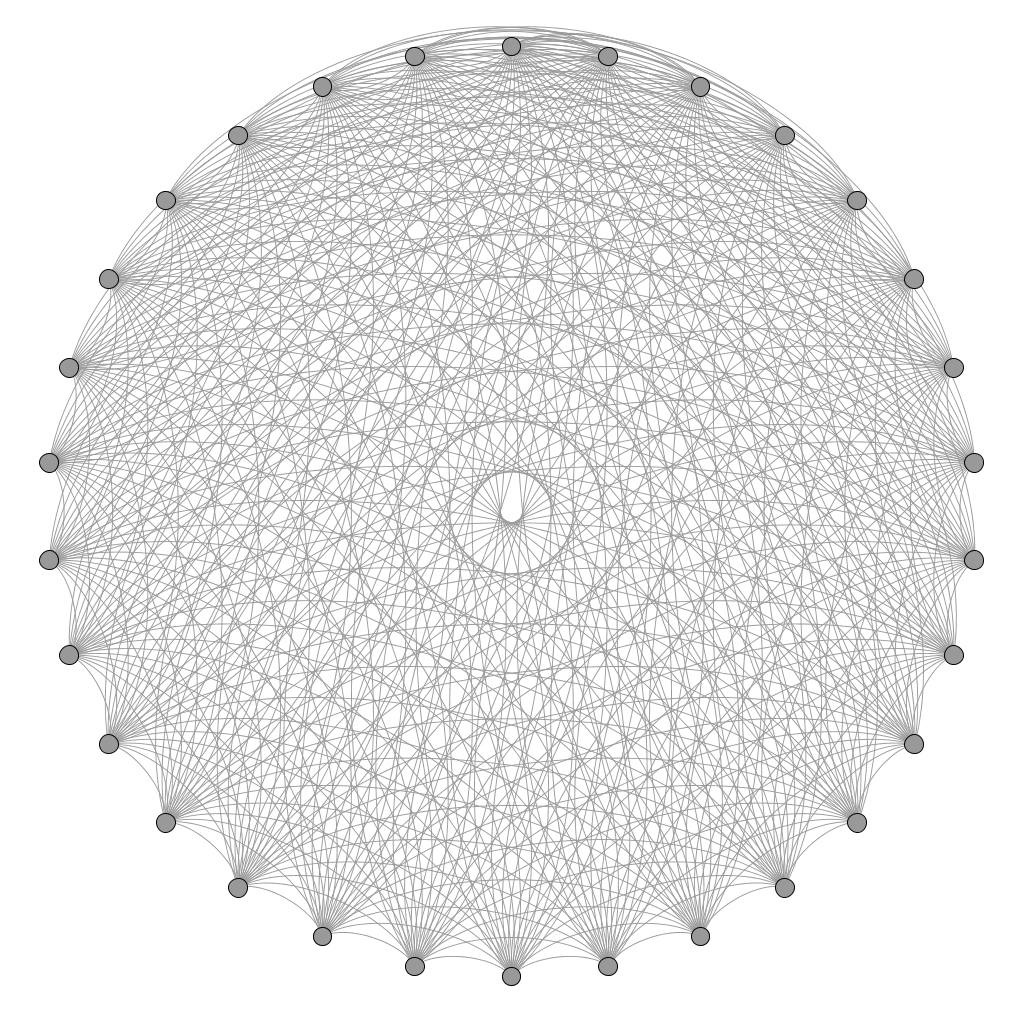
\includegraphics[width=1.0\textwidth, angle=0]{FULLY_CONNECTED_30.png}
	\caption{Fully-Connected topology}
	\label{fig:topology_FULLY_CONNECTED_30}
\end{figure}

\begin{table}[h]
	\centering
	\caption{Network metrics Fully-Connected topology}
	\begin{tabular} { l c r }
		\hline
		Avg. degree & 29 \\
		Avg. path-length & 1 \\
		Avg. clustering coefficient & 1 \\
		Network diameter & 1 \\
		Graph density & 1 \\
		Edge count & $\frac{N(N - 1)}{2}$ \\
		\hline
	\end{tabular}
\end{table}

\section{Half-Fully Connected}
Agents with optimism-factor 0.5 to 1.0 are fully-connected and the others are connected to the agent with the next higher optimism-factor. The agents with highest and lowest optimism-factor are connected too, creating a closed circle.
\medskip
Included to investigate the influence of isolated agents.

\begin{figure}[H]
	\centering
  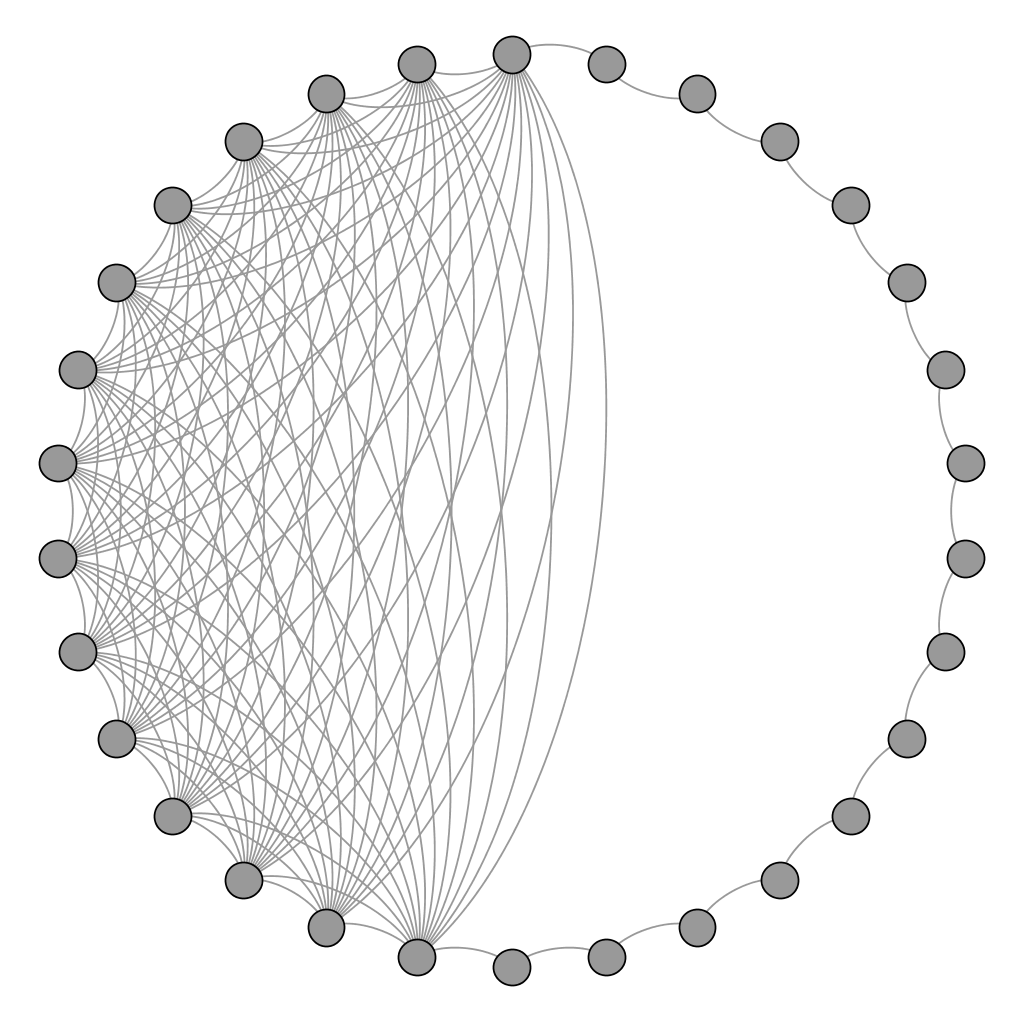
\includegraphics[width=1.0\textwidth, angle=0]{HALFFULLY_CONNECTED_30.png}
	\caption{Half Fully-Connected topology}
	\label{fig:topology_HALFFULLY_CONNECTED_30}
\end{figure}

\begin{table}[h]
	\centering
	\caption{Network metrics Half Fully-Connected topology}
	\begin{tabular} { l c r }
		\hline
		Avg. degree & 8.067 \\
		Avg. path-length & 4.007 \\
		Avg. clustering coefficient & 0.491 \\
		Network diameter & 9 \\
		Graph density & 0.278 \\
		Edge count & $\frac{\frac{N}{2}(\frac{N}{2} - 1)}{2} + \frac{N}{2} + 1$ \\
		\hline
	\end{tabular}
\end{table}

\section{Ascending-Connected}
Each agent is connected to the agent with the next higher optimism-factor. The agents with highest and lowest optimism-factor are not connected thus this network is not a closed circle.
\medskip
Included because it is the most minimal network which satisfies the theory and is therefore the major network of interest throughout the thesis.

\begin{figure}[H]
	\centering
  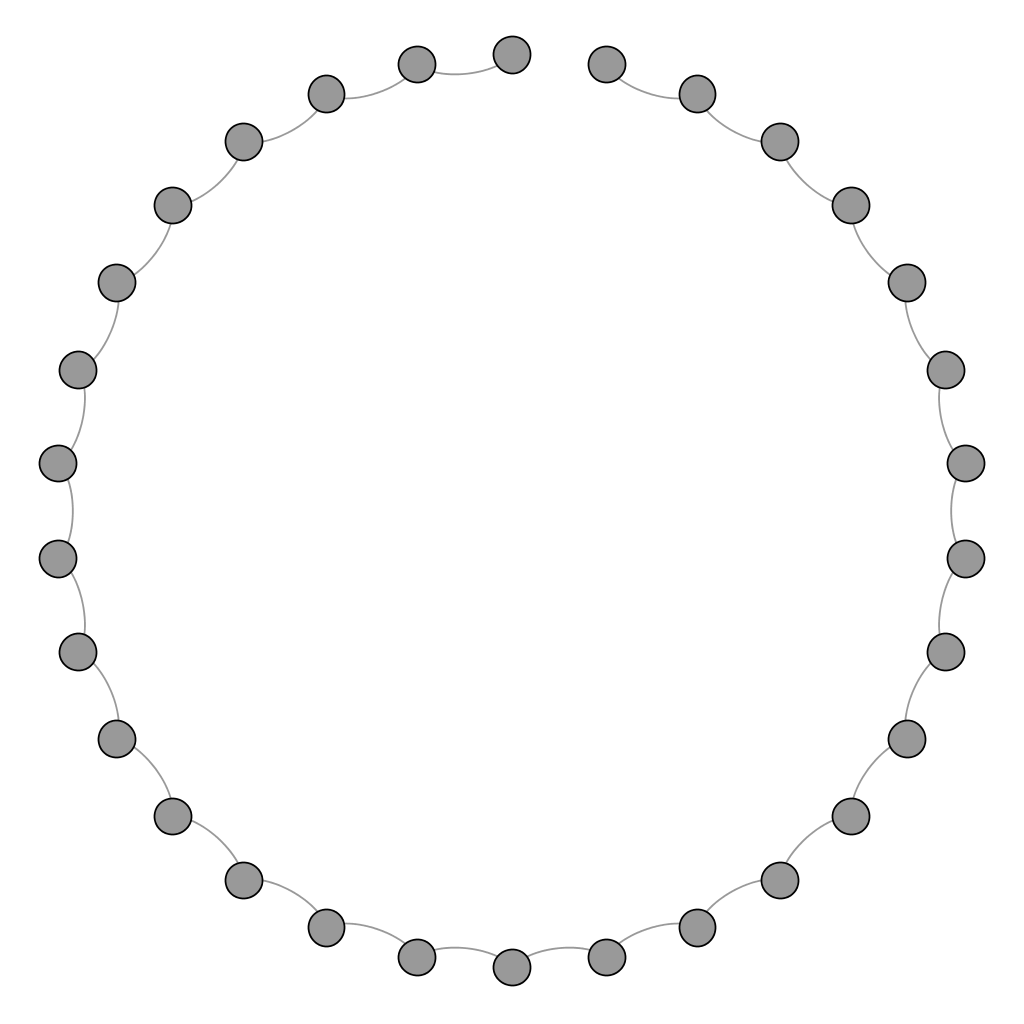
\includegraphics[width=1.0\textwidth, angle=0]{ASCENDING_CONNECTED_30.png}
	\caption{Ascending-Connected topology}
	\label{fig:topology_ASCENDING_CONNECTED_30}
\end{figure}

\begin{table}[h]
	\centering
	\caption{Network metrics Ascending-Connected topology}
	\begin{tabular} { l c r }
		\hline
		Avg. degree & 1.933 \\
		Avg. path-length & 10.33 \\
		Avg. clustering coefficient & 0 \\
		Network diameter & 29 \\
		Graph density & 0.067 \\
		Edge count & $N-1$ \\
		\hline
	\end{tabular}
\end{table}

\section{Ascending-Connected with short-cuts}
\subsection{Full short-cuts}
Each agent is connected to the K next neighbours in the clockwise arrangement. Thus agent N - K + 1 is connected to K - 1 higher optimism-agents and wraps around to the agent with lowest optimism-factor.
\medskip
Included to analyse the influence of increasing connectivity.

\begin{figure}[H]
	\centering
  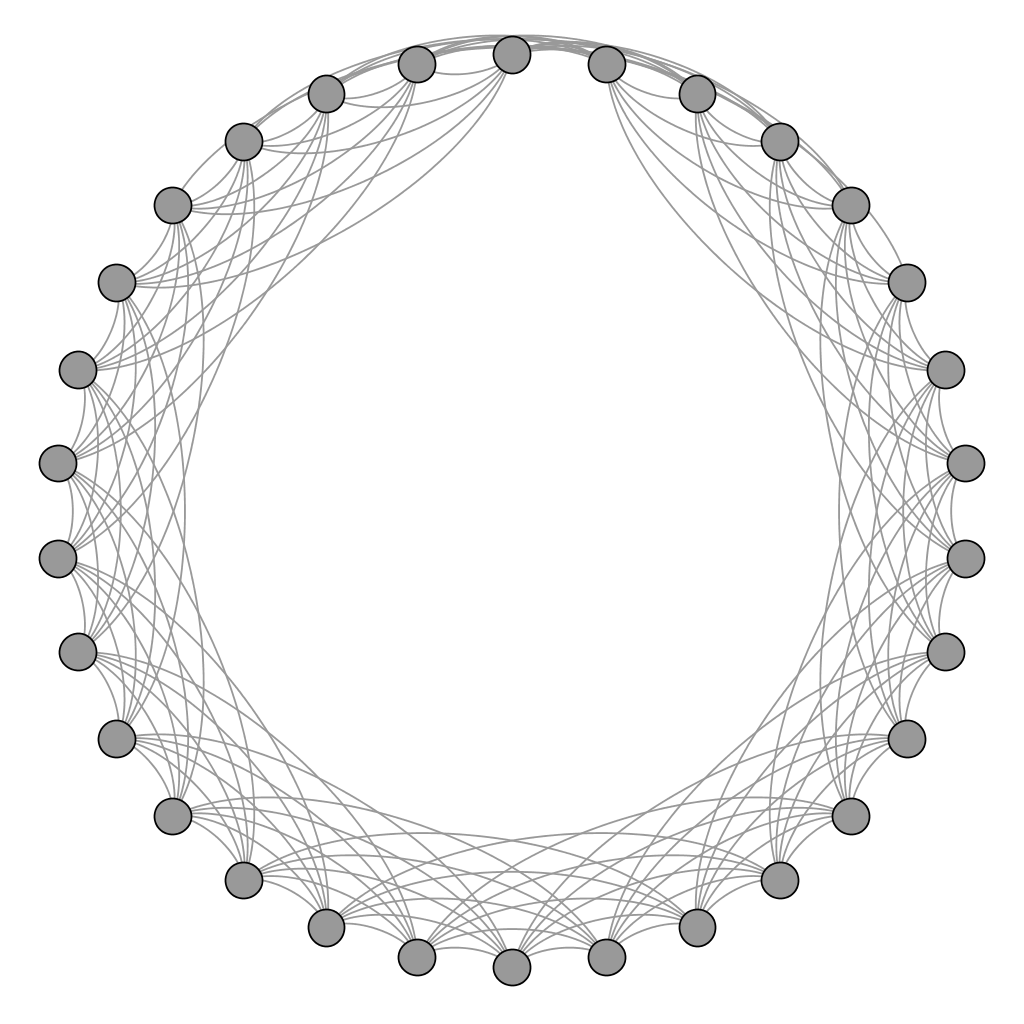
\includegraphics[width=1.0\textwidth, angle=0]{ASCENDING_CONNECTED_FULLSHORTCUTS_5_30.png}
	\caption{Ascending-Connected 5 full short-cuts topology}
	\label{fig:topology_ASCENDING_CONNECTED_FULLSHORTCUTS_5_30}
\end{figure}

\begin{table}[h]
	\centering
	\caption{Network metrics Ascending-Connected 5 full short-cuts topology}
	\begin{tabular} { l c r }
		\hline
		Avg. degree & 10 \\
		Avg. path-length & 1.966 \\
		Avg. clustering coefficient & 0.667 \\
		Network diameter & 3 \\
		Graph density & 0.345 \\
		Edge count & $NK$ \\
		\hline
	\end{tabular}
\end{table}

\subsection{Regular short-cuts}
The topology starts ascending-connected and each agent is additionally connected to one next neighbour in the clockwise arrangement where the distance to the next neighbour is K agents.
\medskip
Included to analyse the influence of trading-links to agents with much higher optimism-factor.

\begin{figure}[H]
	\centering
  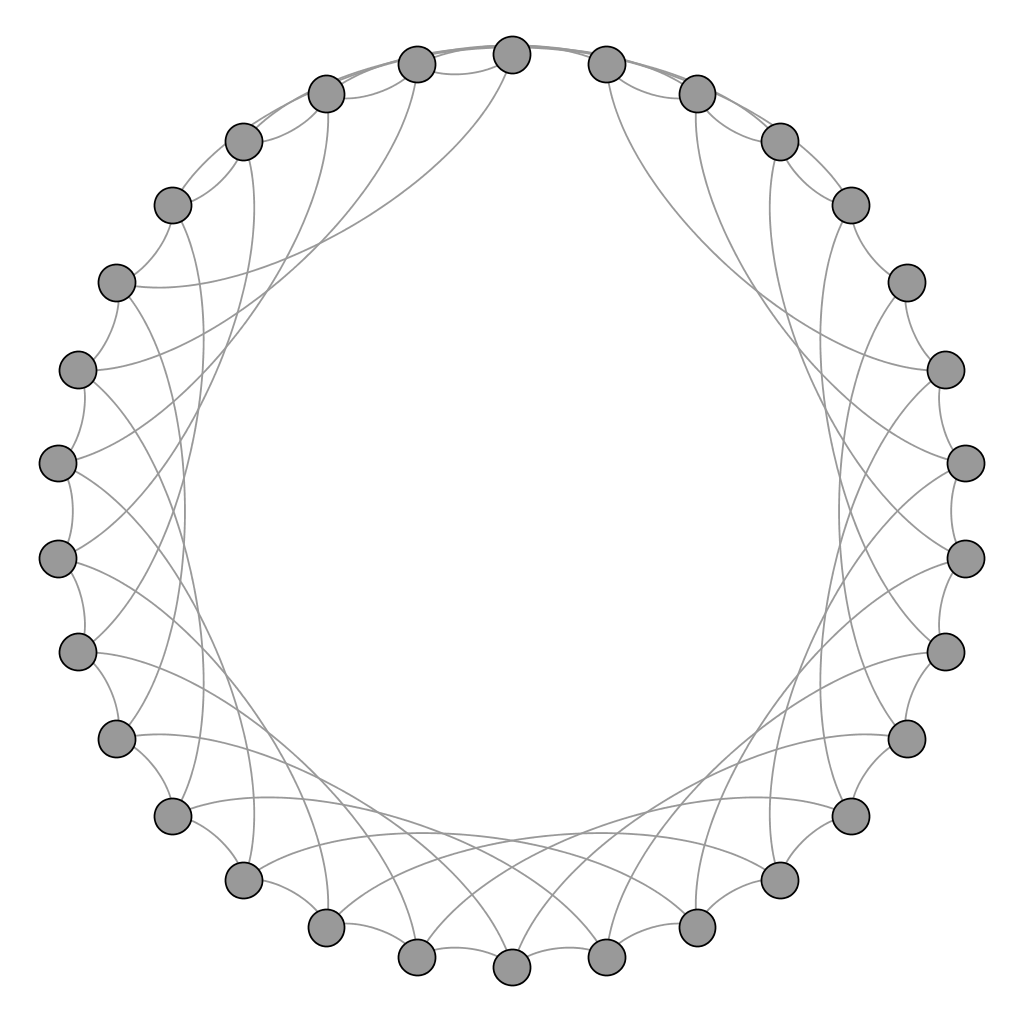
\includegraphics[width=1.0\textwidth, angle=0]{ASCENDING_CONNECTED_REGULARSHORTCUTS_5_30.png}
	\caption{Ascending-Connected 5 regular short-cuts topology}
	\label{fig:topology_ASCENDING_CONNECTED_REGULARSHORTCUTS_5_30}
\end{figure}

\begin{table}[h]
	\centering
	\caption{Network metrics Ascending-Connected 5 regular short-cuts topology}
	\begin{tabular} { l c r }
		\hline
		Avg. degree & 3.867 \\
		Avg. path-length & 2.839 \\
		Avg. clustering coefficient & 0 \\
		Network diameter & 6 \\
		Graph density & 0.133\\
		Edge count & $2N$ \\
		\hline
	\end{tabular}
\end{table}

\subsection{Random short-cuts}
Starting with an ascending-connected network this topology adds one additional short-cut from each agent to another random agent with a given probability where a probability of 0.0 results in only the ascending-connectedness and a probability of 1.0 in each agent having an additional random short-cut. Self-loops and multi-edges are not allowed.
\medskip
Included to analyse the influence of randomness in ascending-connected topologies.

\begin{figure}[H]
	\centering
  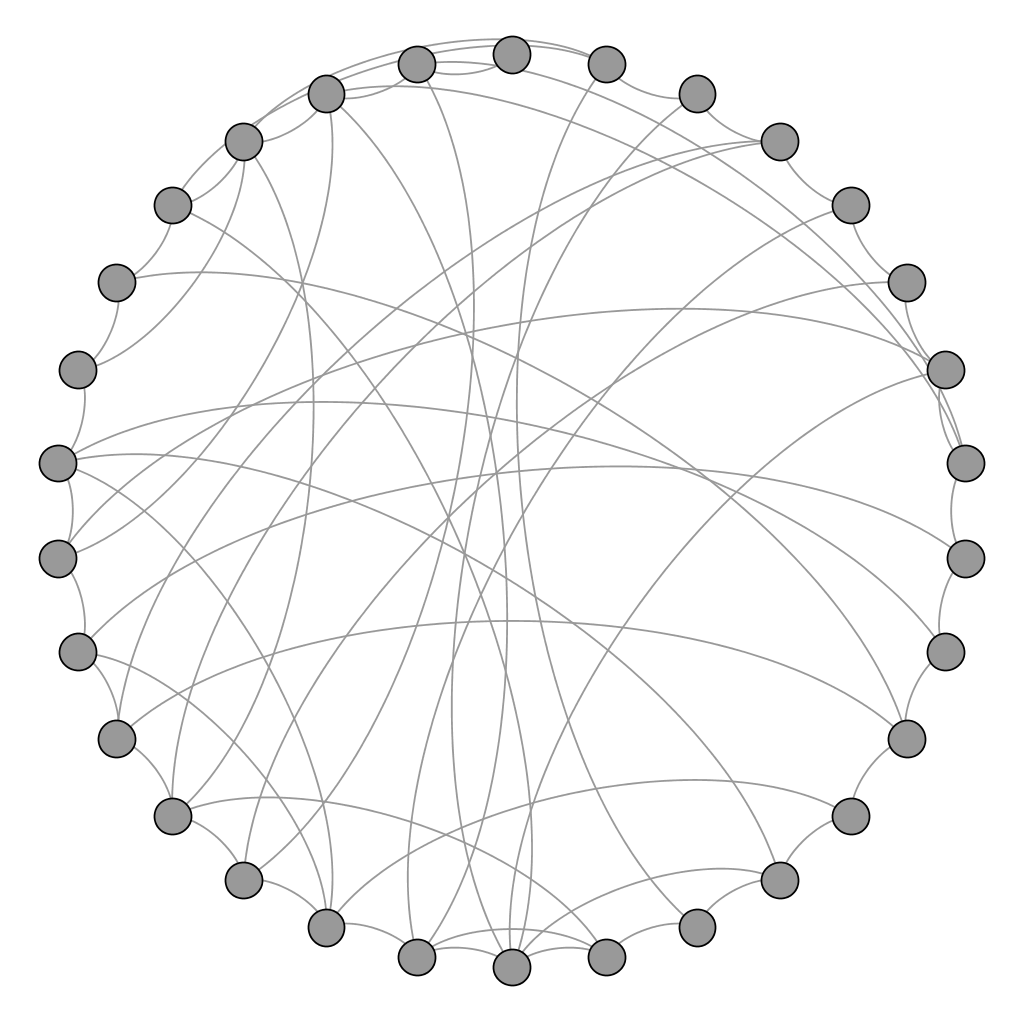
\includegraphics[width=1.0\textwidth, angle=0]{ASCENDING_CONNECTED_RANDOMSHORTCUTS_10_30.png}
	\caption{Ascending-Connected random short-cuts probability 1.0 topology}
	\label{fig:topology_ASCENDING_CONNECTED_RANDOMSHORTCUTS_10_30}
\end{figure}

\begin{table}[h]
	\centering
	\caption{Network metrics Ascending-Connected random short-cuts topology}
	\begin{tabular} { l c r }
		\hline
		Avg. degree & 3.867 \\
		Avg. path-length & 2.506 \\
		Avg. clustering coefficient & 0.056 \\
		Network diameter & 5 \\
		Graph density & 0.133\\
		Edge count & $\min N, \max 2N$ \\
		\hline
	\end{tabular}
\end{table}

\section{Hub-based topologies}
\subsection{3 Hubs}
The agents are separated into 3 groups based upon their optimism-factor. Group 1 ranges from 0.0 to 0.33, group 2 from 0.33 to 0.66 and group 3 from 0.66 to 1.0. All agents within a group are fully-connected where the groups are interconnected between each other through a hub which is the agent with the highest optimism-factor of each group that is: 0.33, 0.66 and 1.0.
\medskip
Included as a point-of-reference as this topology was discussed too in \cite{Breuer2015}.

\begin{figure}[H]
	\centering
  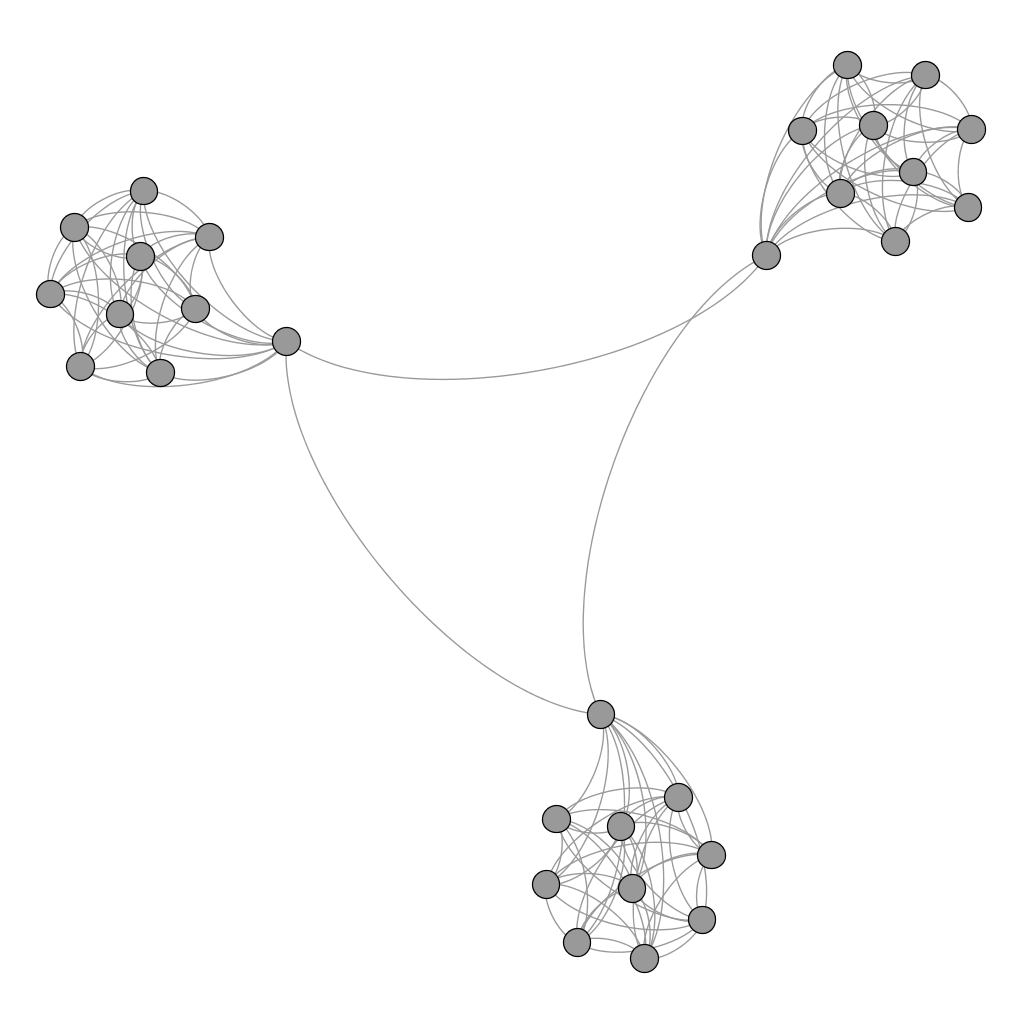
\includegraphics[width=1.0\textwidth, angle=0]{3HUBS_30.png}
	\caption{3 Hubs topology}
	\label{fig:topology_3HUBS_30}
\end{figure}

\begin{table}[h]
	\centering
	\caption{Network metrics 3 Hubs topology}
	\begin{tabular} { l c r }
		\hline
		Avg. degree & 9.2 \\
		Avg. path-length & 2.241 \\
		Avg. clustering coefficient & 0.976 \\
		Network diameter & 3 \\
		Graph density & 0.371\\
		Edge count & $3(\frac{\frac{N}{3}(\frac{N}{3} - 1)}{2}) + 3$ \\
		\hline
	\end{tabular}
\end{table}

\subsection{3 Median Hubs}
There are 3 agents which act as median hubs which are the agent with the median optimism-factor and the next lower and higher ones. All three are connected to each other where the rest of the agents are randomly connected to one hub so that each hub has the same amount of agents.
\medskip
Included to see what happens if all agents can only trade through median agents which are the most active ones in the Fully-Connected topology.

\begin{figure}[H]
	\centering
  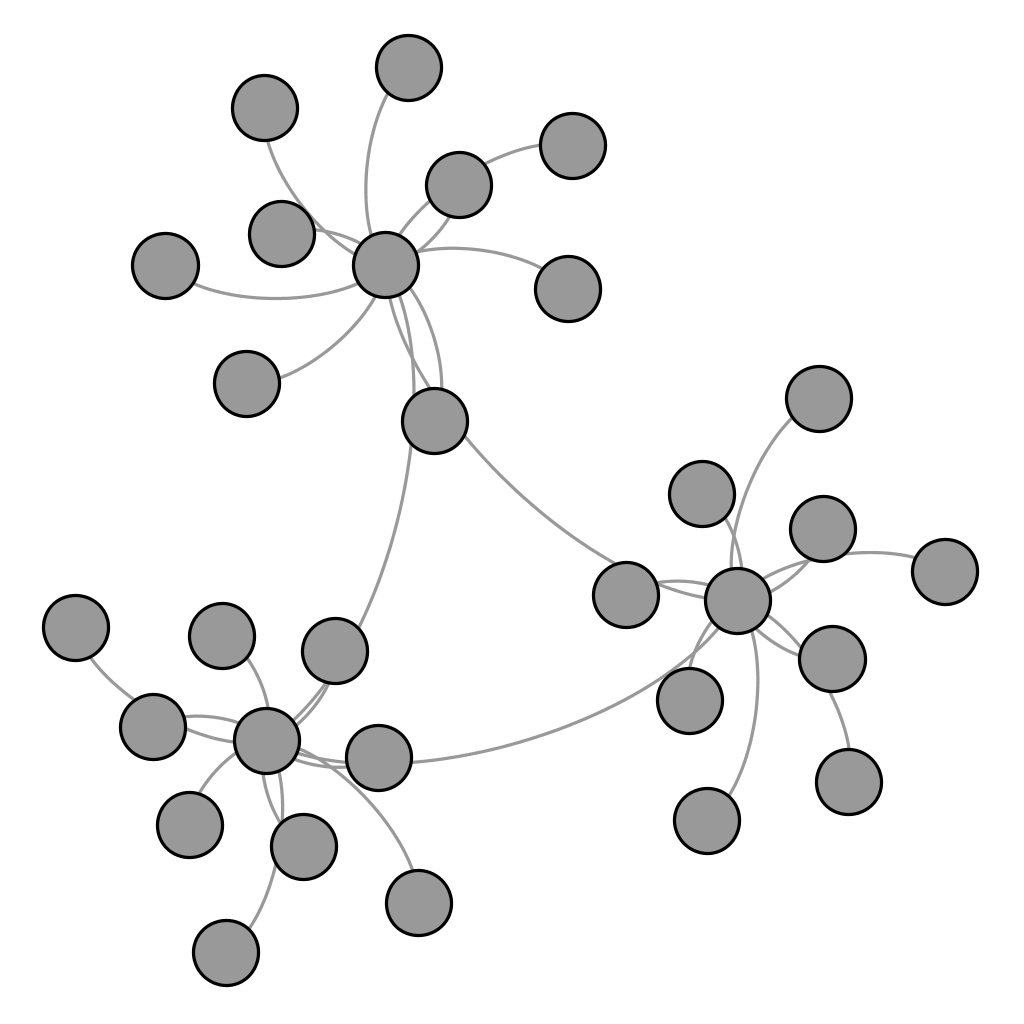
\includegraphics[width=1.0\textwidth, angle=0]{3MEDIANHUB_30.png}
	\caption{3 Median Hub topology}
	\label{fig:topology_3MEDIANHUB_30}
\end{figure}

\begin{table}[h]
	\centering
	\caption{Network metrics 3 Median Hub topology}
	\begin{tabular} { l c r }
		\hline
		Avg. degree & 2 \\
		Avg. path-length & 2.49 \\
		Avg. clustering coefficient & 0.018 \\
		Network diameter & 3 \\
		Graph density & 0.069 \\
		Edge count & $N$ \\
		\hline
	\end{tabular}
\end{table}

\subsection{Median Hub}
All agents are connected to the agent with the median optimism-factor.
\medskip
Included for the same reason as in 3 median hubs but with just one median hub.

\begin{figure}[H]
	\centering
  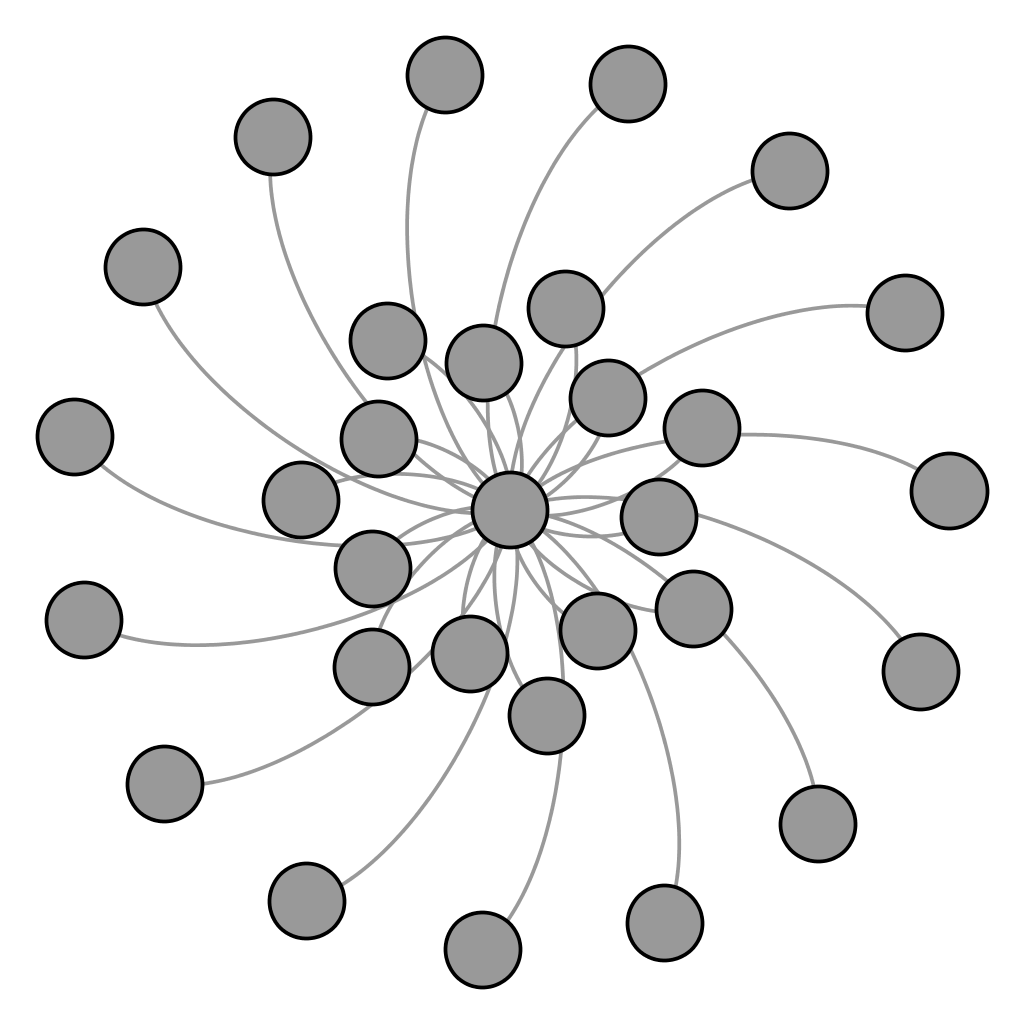
\includegraphics[width=1.0\textwidth, angle=0]{1MEDIANHUB_30.png}
	\caption{Median Hub topology}
	\label{fig:topology_1MEDIANHUB_30}
\end{figure}

\begin{table}[h]
	\centering
	\caption{Network metrics Median Hub topology}
	\begin{tabular} { l c r }
		\hline
		Avg. degree & 1.933 \\
		Avg. path-length & 1.933 \\
		Avg. clustering coefficient & 0 \\
		Network diameter & 2 \\
		Graph density & 0.067 \\
		Edge count & $N-1$ \\
		\hline
	\end{tabular}
\end{table}

\subsection{Maximum Hub}
Looks the same as 1 Median Hub but all edges are connected to the agent with the highest optimism-value. Has thus also the same metrics as the optimism-values have no functional influence on the metrics.
\medskip
Included just out of curiosity and has no real value as it is obviously clear that equilibrium is impossible to be reached in this case.

\section{Small-World and Scale-Free topologies}
\subsection{Erods-Renyi}
Each possible edge is included with a given probability where self-loops and multi-edges are omitted. See section \ref{sec:theory_complexNetworks} for a discussion of this topology.
\medskip
Included to investigate the influence of small-world an scale-free effects upon equilibrium and because of the randomness of the network.

\begin{figure}[H]
	\centering
  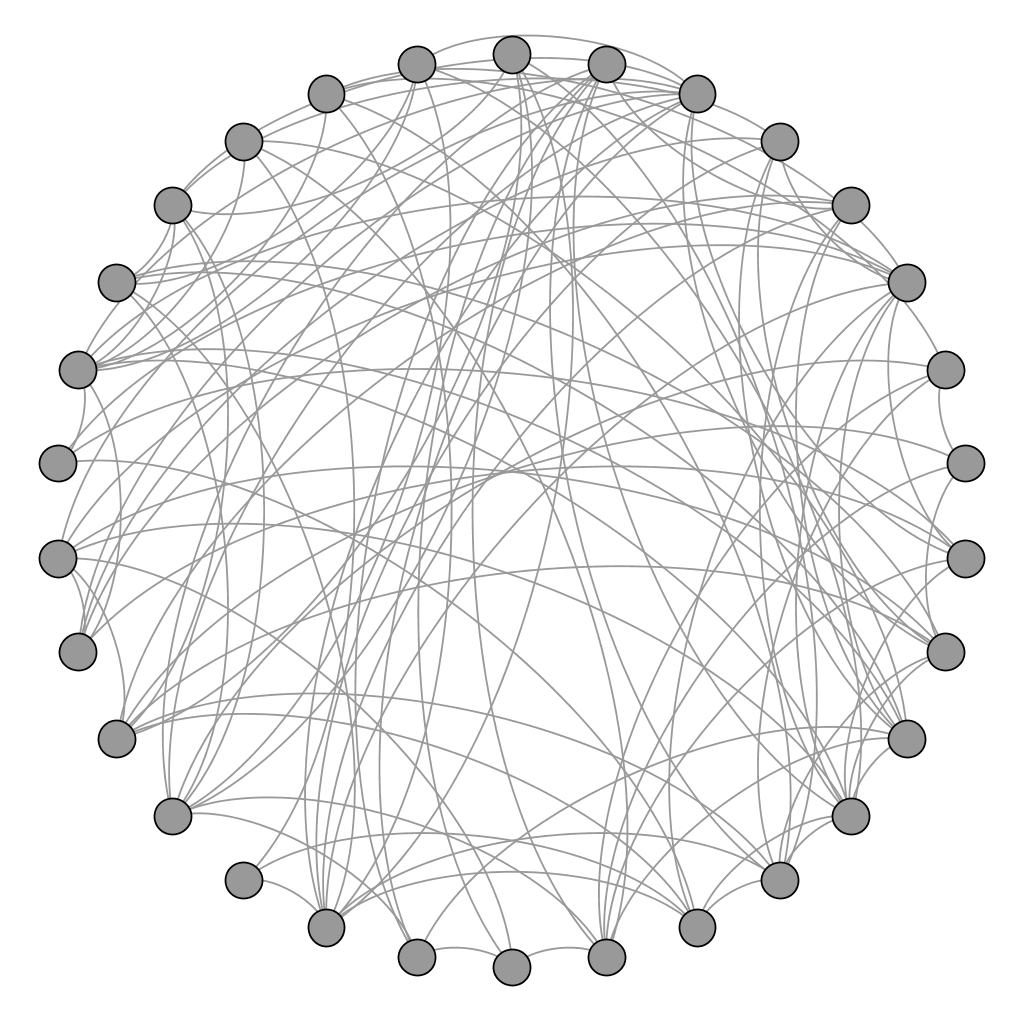
\includegraphics[width=1.0\textwidth, angle=0]{ERDOSRENYI_02_30.png}
	\caption{Erdos-Renyi topology with inclusion-probability of 0.2}
	\label{fig:topology_ERDOSRENYI_02_30}
\end{figure}

\begin{table}[h]
	\centering
	\caption{Network metrics Erdosy-Renyi 0.2}
	\begin{tabular} { l c r }
		\hline
		Avg. degree & 6.8 \\
		Avg. path-length & 1.913 \\
		Avg. clustering coefficient &  0.266 \\
		Network diameter & 3 \\
		Graph density & 0.234 \\
		Connected component & 1 \\
		\hline
	\end{tabular}
\end{table}

\begin{figure}[H]
	\centering
  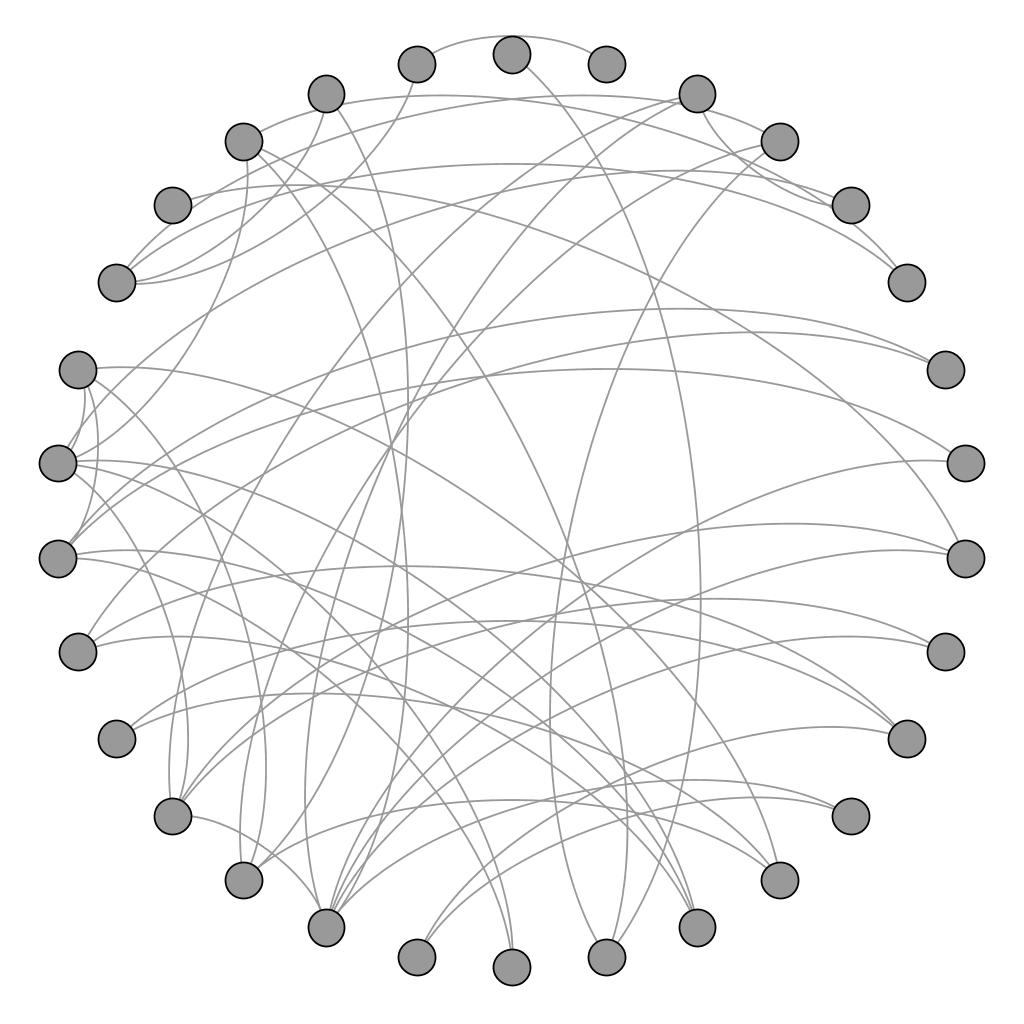
\includegraphics[width=1.0\textwidth, angle=0]{ERDOSRENYI_01_30.png}
	\caption{Erdos-Renyi topology with inclusion-probability of 0.1}
	\label{fig:topology_ERDOSRENYI_01_30}
\end{figure}

\begin{table}[h]
	\centering
	\caption{Network metrics Erdosy-Renyi 0.1}
	\begin{tabular} { l c r }
		\hline
		Avg. degree & 2.933 \\
		Avg. path-length & 3.262 \\
		Avg. clustering coefficient & 0.103 \\
		Network diameter & 7 \\
		Graph density & 0.101 \\
		Connected component & 1 \\
		\hline
	\end{tabular}
\end{table}

\begin{figure}[H]
	\centering
  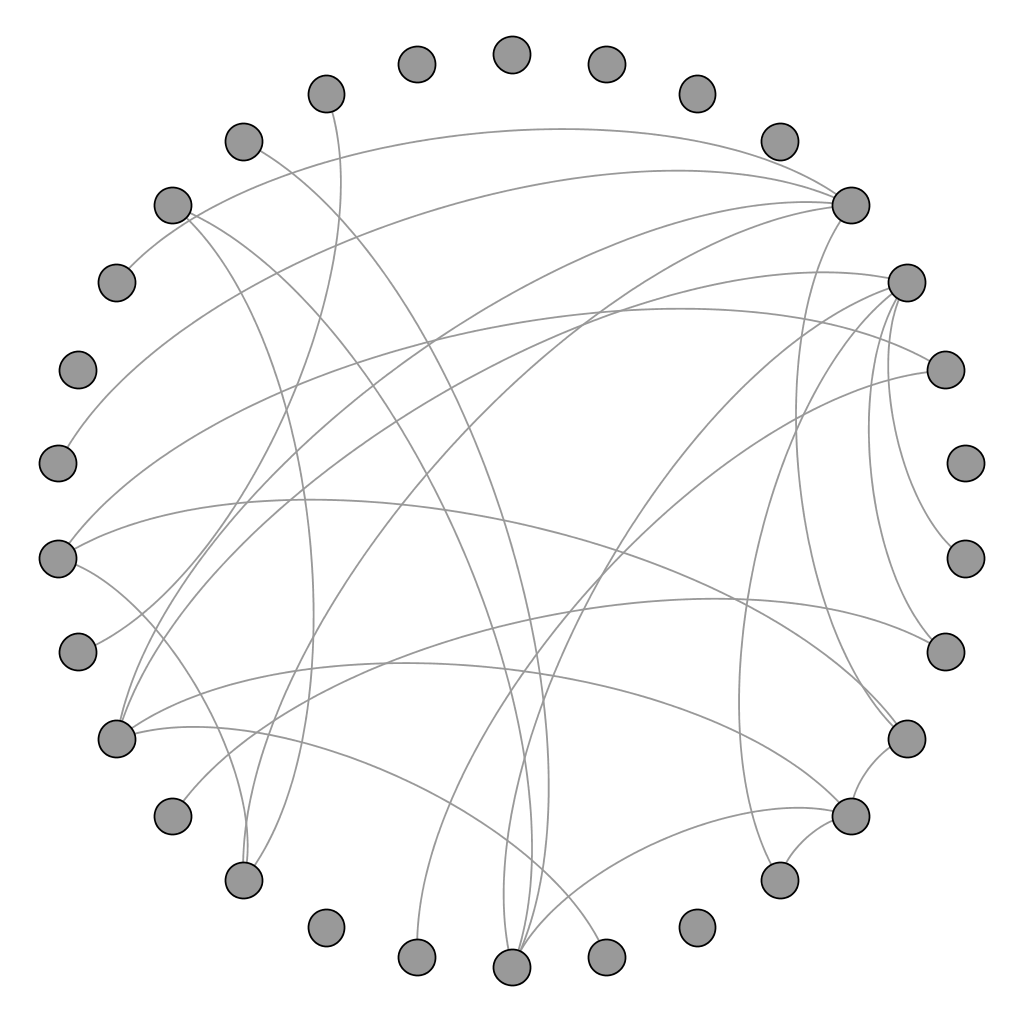
\includegraphics[width=1.0\textwidth, angle=0]{ERDOSRENYI_005_30.png}
	\caption{Erdos-Renyi topology with inclusion-probability of 0.05}
	\label{fig:topology_ERDOSRENYI_005_30}
\end{figure}

\begin{table}[h]
	\centering
	\caption{Network metrics Erdosy-Renyi 0.05}
	\begin{tabular} { l c r }
		\hline
		Avg. degree & 1.6 \\
		Avg. path-length & 3.052 \\
		Avg. clustering coefficient & 0 \\
		Network diameter & 8 \\
		Graph density & 0.055 \\
		Connected component & 11 \\
		\hline
	\end{tabular}
\end{table}

\subsection{Barbasi-Albert}
One starts with m0 nodes and attaches each new node randomly to m existing nodes where the selection-probability of a node depends on its degree. See section \ref{sec:theory_complexNetworks} for a discussion of this topology.
\medskip
Included to investigate the influence of small-world an scale-free effects upon equilibrium and because of the randomness of the network.

\begin{figure}[H]
	\centering
  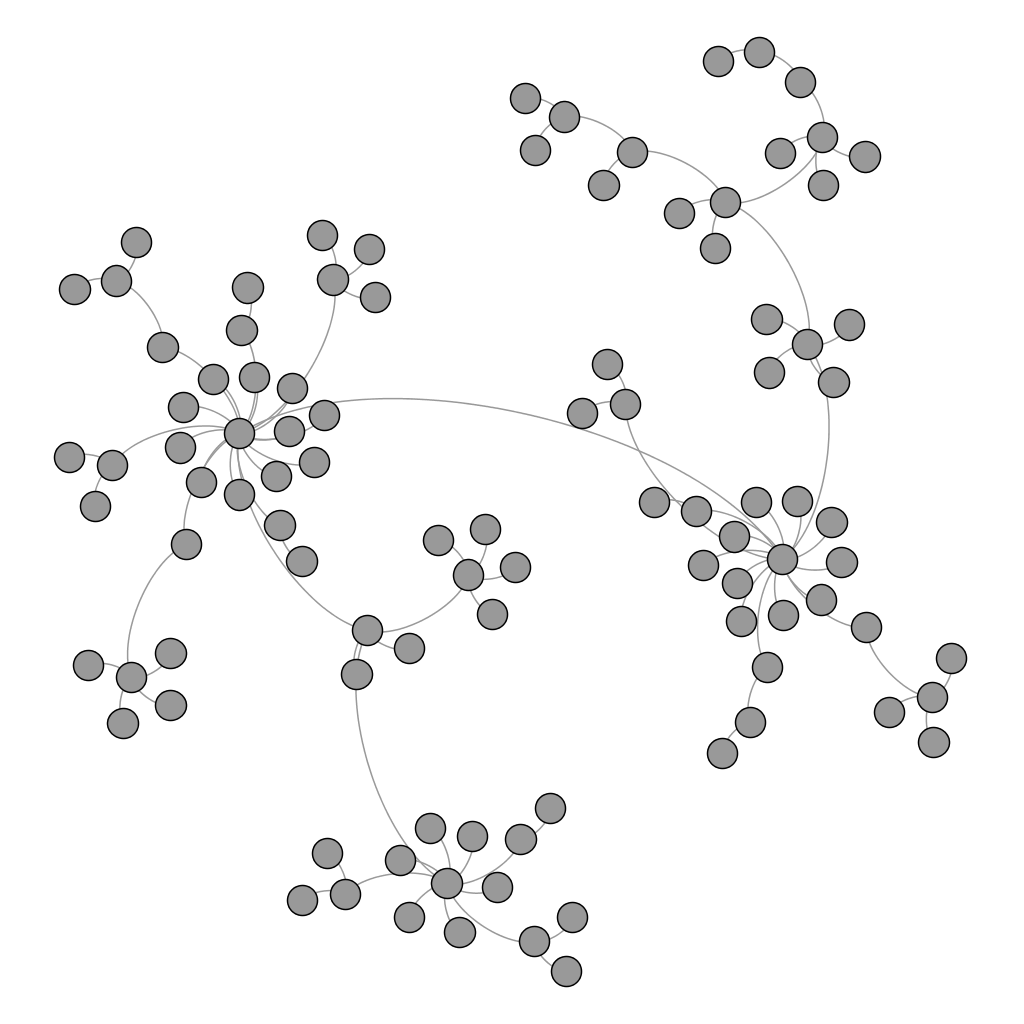
\includegraphics[width=1.0\textwidth, angle=0]{BARBASIALBERT_3_1_30.png}
	\caption{Barbasi-Albert topology with m0=3, m=1}
	\label{fig:topology_BARBASIALBERT_3_1_30}
\end{figure}

\begin{table}[h]
	\centering
	\caption{Network metrics Barbasi-Albert m0=3, m=1}
	\begin{tabular} { l c r }
		\hline
		Avg. degree & 1.98 \\
		Avg. path-length & 4.684 \\
		Avg. clustering coefficient & 0 \\
		Network diameter & 11 \\
		Graph density & 0.02 \\
		\hline
	\end{tabular}
\end{table}

\begin{figure}[H]
	\centering
  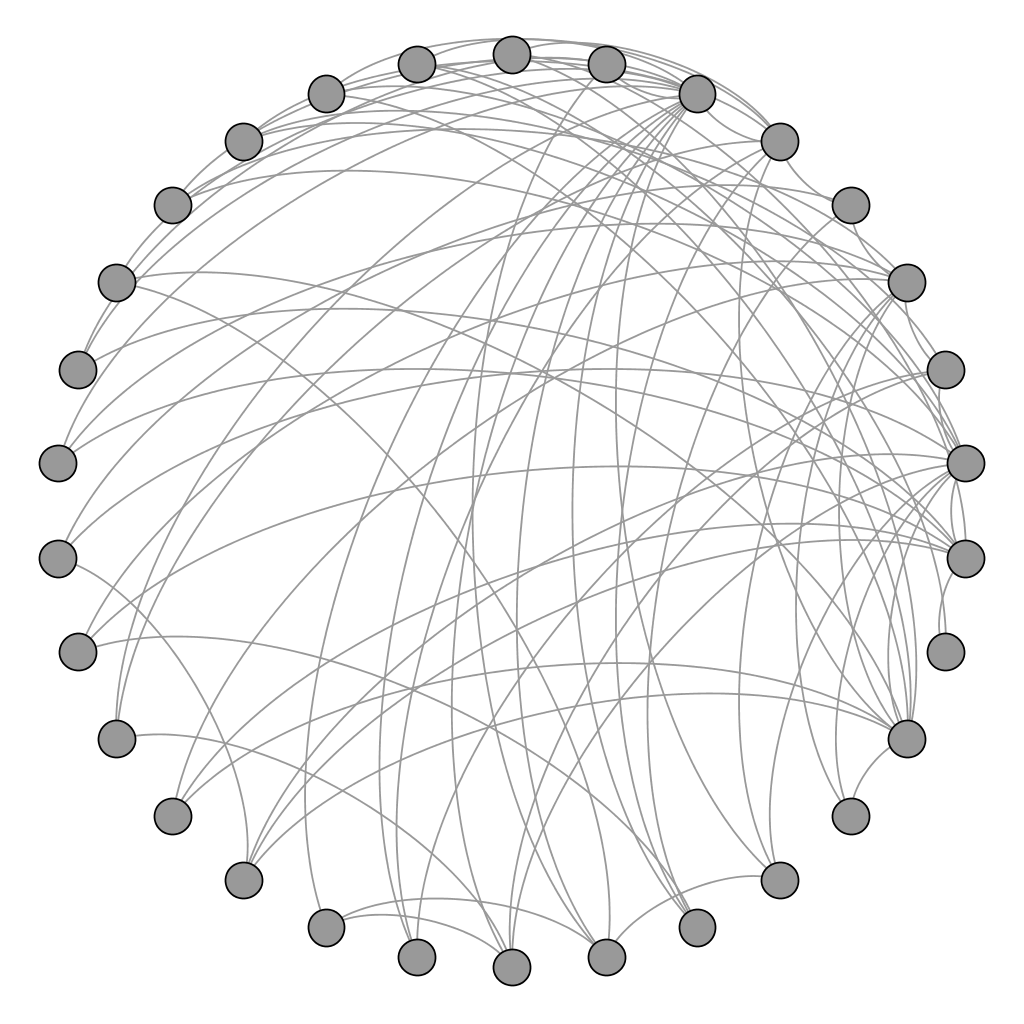
\includegraphics[width=1.0\textwidth, angle=0]{BARBASIALBERT_9_3_30.png}
	\caption{Barbasi-Albert topology with m0=9, m=3}
	\label{fig:topology_BARBASIALBERT_9_3_30}
\end{figure}

\begin{table}[h]
	\centering
	\caption{Network metrics Barbasi-Albert m0=9, m=3}
	\begin{tabular} { l c r }
		\hline
		Avg. degree & 4.733 \\
		Avg. path-length & 2.11 \\
		Avg. clustering coefficient & 0.279 \\
		Network diameter & 4 \\
		Graph density & 0.163 \\
		\hline
	\end{tabular}
\end{table}

\subsection{Watts-Strogatz}
Creates N nodes and connects each to K neighbours and rewires each then existing edge with a probability of 0.2 to a younger node. See section \ref{sec:theory_complexNetworks} for a discussion of this topology.
\medskip
Included to investigate the influence of small-world an scale-free effects upon equilibrium and because of the randomness of the network.

\begin{figure}[H]
	\centering
  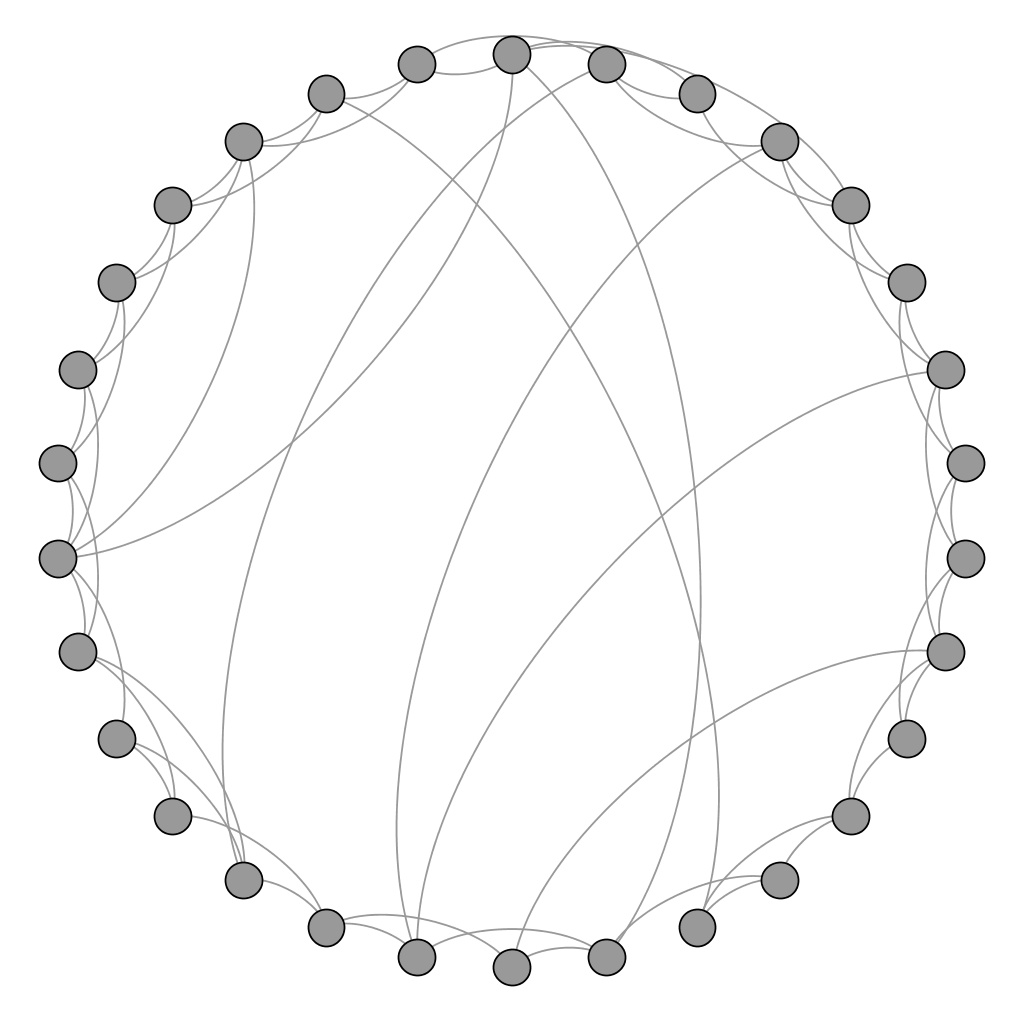
\includegraphics[width=1.0\textwidth, angle=0]{WATTSSTROGATZ_2_02_30.png}
	\caption{Watts-Strogatz topology with k=2, p=0.2}
	\label{fig:topology_WATTSSTROGATZ_2_02_30}
\end{figure}

\begin{table}[h]
	\centering
	\caption{Network metrics Watts-Strogatz k=2, p=0.2}
	\begin{tabular} { l c r }
		\hline
		Avg. degree & 4 \\
		Avg. path-length & 2.883 \\
		Avg. clustering coefficient & 0.259 \\
		Network diameter & 6 \\
		Graph density & 0.138 \\
		\hline
	\end{tabular}
\end{table}

\begin{figure}[H]
	\centering
  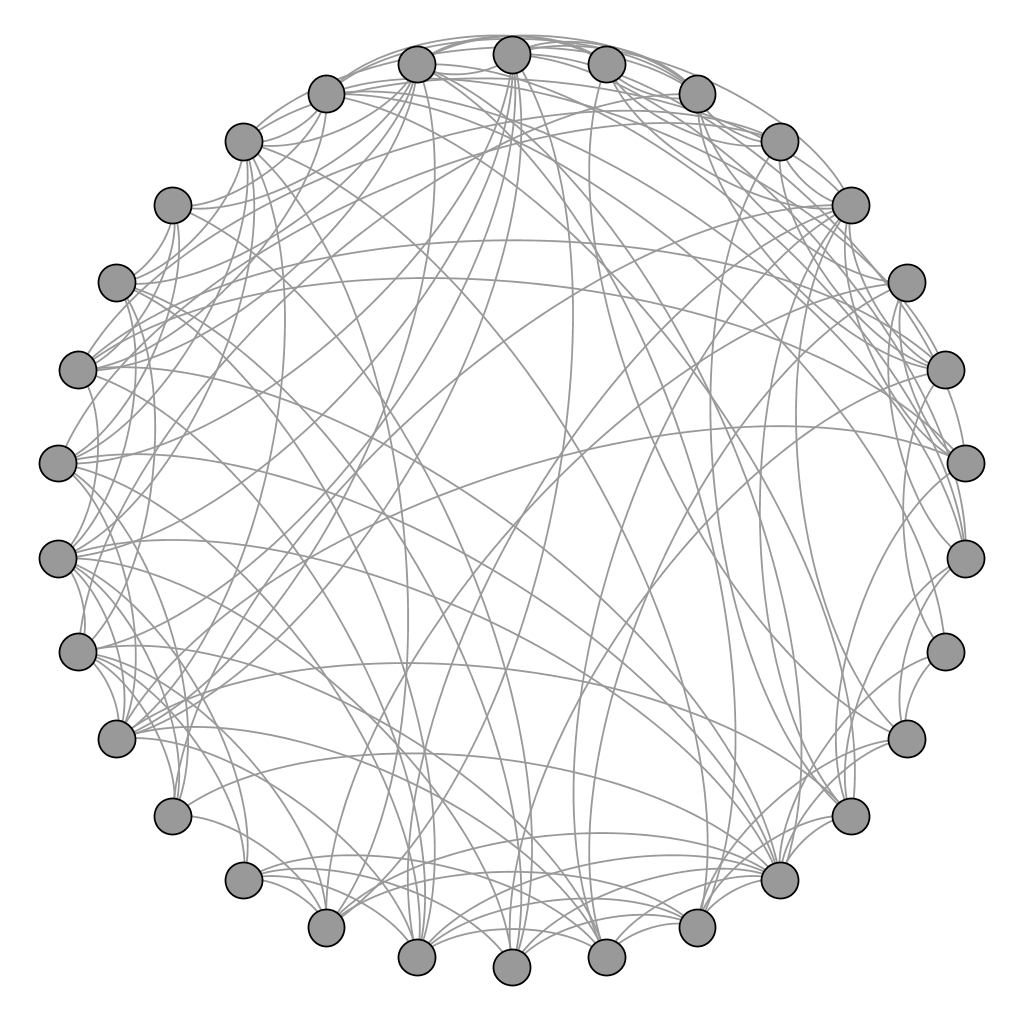
\includegraphics[width=1.0\textwidth, angle=0]{WATTSSTROGATZ_4_05_30.png}
	\caption{Watts-Strogatz topology with k=4, p=0.5}
	\label{fig:topology_WATTSSTROGATZ_4_05_30}
\end{figure}

\begin{table}[h]
	\centering
	\caption{Network metrics Watts-Strogatz k=4, p=0.5}
	\begin{tabular} { l c r }
		\hline
		Avg. degree & 8 \\
		Avg. path-length & 1.823 \\
		Avg. clustering coefficient & 0.241 \\
		Network diameter & 3 \\
		Graph density & 0.276 \\
		\hline
	\end{tabular}
\end{table}

\end{document}